% Stuff for the quads
%% 
\paragraph{Cryogenic Procedures}

\paragraph {First Time Startup Check List.}

See Oxford Instruments User manual for startup check list. \cite{bi:oxf1}

\newpage
\paragraph {Routine Startup Check List Before Energizing Magnets.}

A routine checkout of the quadrupoles by a Hall C Eng. Staff only should include as a minimum
the following:  Magnetic Materials Checks; Vacuum Checks; Cryogenics
and Valve Checks; Electrical and Main Power Supply Checks; and
Computer Control Checks.  A separate check list is included for shift
leaders.  

\subparagraph{Magnetic Materials Checks:}

\begin{itemize}
\item[{[~~~~]}]{Perform a walk around of magnet looking for loose magnetic
materials that could be attracted to the magnet during operation.}
\item[{[~~~~]}]{Check for sensitive electronic equipment that could be
effected or damaged by magnetic fields.}
\item[{[~~~~]}]{Advise any personal near HMS of magnet operations.}
\item[{[~~~~]}]{Ensure that magnetic field signs are posted near magnets
and HMS personnel ladders.}
\end{itemize}


\subparagraph{Vacuum Checks:}

\begin{itemize}
\item[{[~~~~]}]{Verify vacuum via readback on helium page.  (Vac=.25x10${^-6}$ Bar).}
\item[{[~~~~]}]{Check that Helium and Nitrogen Supply valves are at nominal
positions.  Excessive supply valve openings could indicted a higher heat
leak to the magnet cyrogens.}
\item[{[~~~~]}]{Check for condensation and freezing on Outer Vacuum
Chamber (O.V.C.).}
\end{itemize}

\subparagraph{Cryogenics and Valve Checks:}

\noindent On Magnet:

\begin{itemize}
\item[{[~~~~]}]{Visual inspection of magnet cryostat for condensation or frosting.}
\item[{[~~~~]}]{Visual inspection of U-Tubes (connecting distribution can to
magnets) for condensation of frosting.}
\item[{[~~~~]}]{Visual inspection of magnet turret top plate for indications
of any icing other then N2 exhaust pipe.}
\item[{[~~~~]}]{Audible check for any noise indicating a gas leak within main
leads cover housing on top of turret.}
\item[{[~~~~]}]{Check that heater tape is working on top neck of turret can.}
\item[{[~~~~]}]{Visually check all valve actuators for cable connections, LVDT
connections, relative stem position and motor operation.}
\item[{[~~~~]}]{Visual and audible inspection inside distribution box
(located on side of turret can) for leaks.}
\item[{[~~~~]}]{Inspection of lead flow valves for proper operation and position.}
\item[{[~~~~]}]{Check that heaters are set to $\sim$40 C and are working inside
distribution box.}
\item[{[~~~~]}]{Ensure that all manual valves are in correct position for normal
operation.  Helium lead flow/neck flow exhaust valve is to be open. Helium
Cooldown/Warm-up valve is to be closed.}
\end{itemize}

\noindent At Control Rack:

\begin{itemize}
\item[{[~~~~]}]{Verify that helium meter and N2 meter are on and indicating
proper liquid levels. Verify that helium meter and monitor display on helium
page are in close agreement.  (Typically the helium meter reads 4 to 5 percent
higher than monitor.)}
\item[{[~~~~]}]{Verify that nitrogen meter and monitor display on nitrogen
page agree with each other.}
\item[{[~~~~]}]{Check temperatures on monitor temperature screen.}
\item[{[~~~~]}]{Check temperatures on monitor helium screen. (4.4-4.7 K)}
\item[{[~~~~]}]{Check temperatures on monitor nitrogen screen. (77.- 80 K)}
\item[{[~~~~]}]{Check helium pressure on monitor reads about 1.34 Bar.}
\item[{[~~~~]}]{Check neck flow and current lead flows are reading near 10
L/min. with no current.  The current lead flow valves position should read
near 10\% open.}
\item[{[~~~~]}]{Make sure that PSU is disabled, Type on command line
PSU:SETCUR:1023.0.  Verify that lead flow readings increase to around 24
L/min. and that valve position readings increase.}
\item[{[~~~~]}]{Type on command line PSU:SETCUR:0.0. Verify that lead flow
valves return to previous valves (10L/min. at 10\% open).}
\item[{[~~~~]}]{Check the following valves for control and read back by opening
and closing the valve by 5\%(max.).}

\begin{center}
  \begin{tabular}{ll}
Valve 8	& Helium Cold Supply Top Fill		\\
Valve 6	& Helium Cold Supple Bottom Fill	\\
Valve 13& Helium Cold Return			\\
	& (Verify that Helium Pressure changes  \\
        &  with valve opening and closing)      \\
Valve 3	& LN$_2$ Supply Top Fill		\\
  \end{tabular}
\end{center}
\item[{[~~~~]}]{All other valves should be at a hard set -i.e. -6\% to
-3\% except the nitrogen check valve, \#19, which should read OPEN.}
\item[{[~~~~]}]{Go to trend page and verify that nitrogen and helium levels
have been maintained at proper levels for the last 24
hours.  (Helium level 75\%, Nitrogen Level 70\% to 80\%).}
\end{itemize}


At a remote terminal logged into a cdaq2 account:

\begin{itemize}
\item[{[~~~~]}]{Check HMS data logging program for the following:

Properly logging HMS and CHL data.

HMS transfer line temperature probes are correct.  (Displayed as
Carriage Temperatures).}
\begin{center}
  \begin{tabular}{lll}
T1	& 5.4 to 5.5 K	& Helium Supply Temp. 1	\\
T2	& 5.5 to 5.8 K	& Helium Supply Temp. 2	\\
T3	& 78 to 180 K	& Nitrogen  trace line.	\\
T4	& 4.4 to 4.6 K	& Dipole helium return.	\\
T5	& 5.4 to 5.6 K	& Dipole helium inlet.	\\
  \end{tabular}
\end{center}
\item[{[~~~~]}]{Check that CHL data is reasonable.}
\begin{center}
  \begin{tabular}{lll}
CFI1139 & 5.0 to 10.0 g/s & He supply Flow \\
CPI671T & 2.4 to 2.8 atm & He supply Pressure \\
CPI9521 & 1.14 to 1.17 atm & He return Pressure \\
CTD671T & 5.2 to 5.6 K & He supply Temp. 1 \\
CTD9521 & 5.3 to 5.7 K & He supply Temp. 2 \\
\end{tabular}
\end{center}
\item[{[~~~~]}]{Check with CHL about their present and future status.}
\end{itemize}


\subparagraph{Electrical and Main Power Supply Checks:}

\begin{itemize}
\item[{[~~~~]}]{480V Main circuit Breaker:  should be locked OFF
before opening Main Power Supply cabinet doors.}
\item[{[~~~~]}]{Individual 208V magnet circuit breakers are in the on
position.  (Located within service lug near center pivot.
Q1:\hskip0.3in ,Q2:\hskip0.3in ,Q3:\hskip0.3in ).}
\item[{[~~~~]}]{Check for Magnet short to ground. Record resistance measurements.}
\item[{[~~~~]}]{Visual inspection of main current leads connection inside of
Main Power Supply. Check for loose connections.}
\item[{[~~~~]}]{Control computer up and running.}
\item[{[~~~~]}]{Quench Detector powered and no interlocks.}
\item[{[~~~~]}]{Interface Unit powered and no interlocks.}
\item[{[~~~~]}]{Control rack power supplies operating  (Three power supplies
located at bottom of rack).}
\item[{[~~~~]}]{Energy dump rack powered and interlock cable connected. Test
Energy dump switch by unplugging interlock cable. Reconnect interlock cable
and reset dump switch. Clear interlocks at control rack.}
\item[{[~~~~]}]{Repeat energy dump test by unplugging power cord to rack.
Clear interlocks.}
\item[{[~~~~]}]{UPS power verified within control rack.}
\item[{[~~~~]}]{Check LCW supply and return pressures as well as flow rate.
[Near pivot].}
\item[{[~~~~]}]{Ensure that cooling water is turned on to power supply.}
\item[{[~~~~]}]{Check for water leaks within power supply unit.}
\item[{[~~~~]}]{Close all doors and cabinets.}
\item[{[~~~~]}]{Turn on 480V main circuit breaker.}
\item[{[~~~~]}]{Ensure that the power enable switch (located in Hall~C
counting room) is enable.}
\item[{[~~~~]}]{Turn on power supply switch.}
\item[{[~~~~]}]{Check all interlocks displayed on power supply led display.
Clear interlocks via front panel reset button on power supply unit.}
\item[{[~~~~]}]{Turn off water supply to power supply. Check that water
flow interlock comes on. Turn water back on and reset interlock.}
\item[{[~~~~]}]{Open front door of PSU. Check door interlock. Secure door and
reset interlock.}
\item[{[~~~~]}]{Test Panic button on front of PSU. Reset.}
\end{itemize}

\subparagraph{Computer Control Checks:}

\begin{itemize}
\item[{[~~~~]}]{Clean PC's Dust filter.}
\item[{[~~~~]}]{Go to Interlock screen. Verify and clear any interlocks.}
\item[{[~~~~]}]{Go to Power supply screen. Enable Power supply control by
typing in command line ``Mode:Normal".}
\item[{[~~~~]}]{Type on command line ``PSU:Remote".}
\item[{[~~~~]}]{Type on command line ``PSU:Reset".}
\item[{[~~~~]}]{Type on command line ``PSU:On".}
\item[{[~~~~]}]{Observe if magnet ``ON" lights (magenta flashing lights) are
activated on HMS carriage.}
\item[{[~~~~]}]{Go to Coil Monitor screen.}
\item[{[~~~~]}]{Type on command line ``Psu:setcur:100.0"}
\item[{[~~~~]}]{Observe coil voltages and current lead voltage readback. Note
any unusual behavior.}
\item[{[~~~~]}]{Activate the shutdown icon on power supply screen.}
\item[{[~~~~]}]{Clear interlocks and turn PSU back on.}
\item[{[~~~~]}]{Test polarity reversing switching.}
\item[{[~~~~]}]{Type on command line ``PSU:standby".}
\item[{[~~~~]}]{Type on command line ``mode:standby".}
\item[{[~~~~]}]{Pass control of magnet up to counting house.}
\item[{[~~~~]}]{Verify safe operation of control system from counting house.}
\end{itemize}

\vspace{0.5in}
\hspace*{3.5in}{\underline{~~~~~~~~~~~~~~~~~~~~~~~~~~~~~~~~~}}
\newline
\hspace*{3.5in}{Signature~~~~~~~~~~~~Date}


\newpage
\paragraph{Long Term Shutdown - Restart Check List:}

A long term shutdown shall be defined if any of the following
conditions is satisfied: a period of time that exceeds 2 months without
having energized the magnets, after a magnet has been warmed to room
temperature and then re-cooled to operating temperatures or after a
replacement/repair of a major piece of equipment directly related to the
operation of the magnet, such as energy dump, main power supply, quench
detector, electronic interface unit, or control PC.  The check out list for
operating the magnets after a long term shut down shall include:

\begin{itemize}
\item[{[~~~~]}] {To be performed by approved Hall C engineering staff.}
\item[{[~~~~]}] {Off line test and confirmation of repaired or
replacement (R\&R) part (if warranted).}
\item[{[~~~~]}] {Test and verification of connections between R\&R
part and the control system.}
\item[{[~~~~]}] {Verification of all electrical and sensor
connections within control rack.}
\item[{[~~~~]}] {Perform a full interlock test.}
\item[{[~~~~]}] {Quench Detector threshold levels tested via the
quench detector test boards.}
\item[{[~~~~]}] {Perform the Routine Startup Check list.}
\item[{[~~~~]}] {Perform a full current ramp [200 amps steps] and
soak for one hour
at full current for each polarity. Record voltages for the coil, leads, and
the power supply output voltage. Ramp magnet down.}
\end{itemize}

\vspace{0.5in}
\hspace*{3.5in}{\underline{~~~~~~~~~~~~~~~~~~~~~~~~~~~~~~~~~}}
\newline
\hspace*{3.5in}{Signature~~~~~~~~~~~~Date}

\newpage
\paragraph{Annual Check List:}

On an annual basis a complete check out of the control system
shall be done. This should include at the least the following checks by a
qualified operator:

\begin{itemize}
\item[{[~~~~]}] {A complete test of interlocks and protection devices.~\cite{bi:oxf2,bi:danf}}
\end{itemize}

At the control rack test the following:

\begin{itemize}
\item[{[~~~~]}]{Watchdog.}
\item[{[~~~~]}]{He Neck flow.}
\item[{[~~~~]}]{He reservoir low.}
\item[{[~~~~]}]{He pressure high.}
\item[{[~~~~]}]{N2 pressure high.}
\item[{[~~~~]}]{CEBAF shutdown.}
\item[{[~~~~]}]{Trim Coil Quench.}
\item[{[~~~~]}]{Dump Switch open.}
\item[{[~~~~]}]{Current Lead overvoltage.}
\item[{[~~~~]}]{Main Coil overvoltage.}
\end{itemize}


At the power supply test:

\begin{itemize}
\item[{[~~~~]}]{Control Rack I/L.}
\item[{[~~~~]}]{Panic / Door I/L. (Panic switch)}
\item[{[~~~~]}]{Panic / Door I/L. (Door switch)}
\item[{[~~~~]}]{MPS waterflow.}
\item[{[~~~~]}]{MPS overtemp.}
\item[{[~~~~]}]{Phase Failure.}
\item[{[~~~~]}]{Reg. Module Failure.}
\item[{[~~~~]}]{Max. Current Set.}
\item[{[~~~~]}]{Transducer Fail.}
\item[{[~~~~]}]{Transistor Failure.}
\item[{[~~~~]}]{Fuse Failure.}
\end{itemize}

\begin{itemize}
\item[{[~~~~]}] {Quench detector threshold levels tested and values recorded.}
\item[{[~~~~]}] {Test of backup temperature probes and voltage taps.}
\item[{[~~~~]}] {Control PC performance checked out and recorded.}
\item[{[~~~~]}] {PC's ADC tested.}
\item[{[~~~~]}] {Verification of all electrical and sensor connections within control
 rack.}
\item[{[~~~~]}] {Inspection of power lead cables within power supply, energy dump
rack and along cable tray up to magnet connection.}
\item[{[~~~~]}] {Inspection of signal cables.}
\item[{[~~~~]}]  {Perform a full valve stroke of all cryogenic valves.}
\item[{[~~~~]}] {Check U-tubes vacuum.}
\item[{[~~~~]}] {Re-calibrate pressure gauges.}
\item[{[~~~~]}] {Inspection of Safety devices (rupture disk, relief valves, parallel
plates).}
\item[{[~~~~]}] {Backup check of O.V.C. vacuum via C.E.B.A.F.'s cold cathode gauges
and/or a RGA system.}
\item[{[~~~~]}] {Visual inspection of control rack's internal electrical components}
\item[{[~~~~]}] {Visual inspection of energy dump rack's internal electrical
components and connections.}
\item[{[~~~~]}] {Record energy dump's resistance.}
\item[{[~~~~]}] {Record power lead cables resistance.}
\item[{[~~~~]}] {Test trim coils.}
\end{itemize}
%\newpage
Perform Maintenance on main power supply as describe by Danfysik 
power supply (See Magnet Power Supply System 8000 section 5, page 77 to 78.).
\begin{itemize}
\item[{[~~~~]}] {Verify power supplies current limitation settings (front panel and
internal settings).}
\item[{[~~~~]}] {Check for short to ground. Record resistance measurements.}
\item[{[~~~~]}]  {Do a routine start check list.}
\item[{[~~~~]}] {Perform a slow discharge of magnet at full field. Record magnet
voltage vs time. Repeat with opposite polarity.}
\item[{[~~~~]}] {Perform a fast discharge of magnet at full field. Record magnet
voltage vs time. Repeat with opposite polarity.}
\item[{[~~~~]}]  {Clean and dust components.}
\end{itemize}

\vspace{0.5in}
\hspace*{3.5in}{\underline{~~~~~~~~~~~~~~~~~~~~~~~~~~~~~~~~~}}
\newline
\hspace*{3.5in}{Signature~~~~~~~~~~~~Date}

\begin{obsolete}
\paragraph{Magnet Selection}

The superconducting magnet keyboard and video signals are transmitted to
the Counting House via a switchable link.  The video is amplified and
the Counting House quality is as good as that in Hall~C.  The keyboard
commands are somewhat slower than the local keyboards but usually work
properly.  Occasionally junk commands (usually a string of dots) appear
in the quad dialogue box due to the switching.  The quads usually ignore
all bad commands.

\paragraph{Selecting a magnet}

\begin{center}
\begin{tabular}{lll}
\multicolumn{3}{c} {Sequence of keystrokes...How to select a magnet.}\\
\hline
        &Press and hold &``Num lock"	\\
        &Press and hold	&``minus (--)"	\\
        &Release	&``minus (--)"	\\
        &Release	&``Num lock"	\\
        &Press one of	&``A" for Q1	\\
        &  	&``B" for Q2	\\
        &		&``C" for Q3	\\
        &		&``D" for Dipole	\\
        &Press		&``Return"	\\
  \end{tabular}
\end{center}

\paragraph{Using the keyboard}

\begin{description}
\item{\bf 1~}\hskip0.1in The quadrupoles use only normal keyboard operations
such as
Alphanumeric keys, cursor keys, and return for selection.  The ``Esc"
(escape) key is also used for menu selection.  The ``Home" key is used to
move from the upper screen to the lower screen.  ({\bf Note:} Num Lock
must not be on to use home key on Num pad).
\item{\bf 2~}\hskip0.1in The dipole keyboard has a built in track ball that
is not
emulated in the Counting House.  You must use the cursor keys and then
type ``exec" (execute) to make a selection, i.e. to plot a graph, select
from a screen menu or to access a valve control menu.  The dipole makes
extensive use of the ``f" keys and a menu is always on the bottom of the
screen.
\item{}\hskip0.3in {\bf Note:  F8 exits the program and saves the trend data}
\item{}\hskip0.3in The alpha numeric keys are used as usual although the PDS
(dipole interface) is built around ``point and click" so only an occasional
number entry is required.
\item{\bf 3~}\hskip0.1in Saving Data
\item{\bf 3.1~}\hskip0.1in The quad system saves data for up to 1 week
without operator
intervention. The data must be transferred to floppy disc to ensure
that it is not overwritten.
\item{}\hskip0.3in {\bf Note:} The quad (Paragon) system start command is
``CEBAF"
\medskip
\item{\bf 3.2~}\hskip0.1in The dipole does not automatically save data without
assistance from an operator.  The dipole has a fast ($\sim$ 2 hour)
buffer and a slow ($\sim$ 1 week) buffer.  The data is stored in 1
day/20 min subsets.  The data can be saved by typing
\end{description}

\begin{center}
  \begin{tabular}{cccc}
	&FREEZE/TR=0 	&	& (RETURN)	\\
	&		& and	&		\\
	&FREEZE/TR=1	&	& (RETURN)	\\
  \end{tabular}
\end{center}

\begin{description}
\item{}\hskip0.3in The data will also be saved by pressing the F8 key to
exit the
PDS program. You must type ``HMS" (return) at the DOS prompt to restart.
Saving the data is a good idea but exiting the program is not,
therefore exit (F8) only in desperation.
\item{\bf 4~}\hskip0.1in Rebooting
\item{}\hskip0.3in It is possible to perform a soft boot ``CTRL - ALT - DEL"
from the Counting House keyboard.  The remote system has a hard time
transmitting this, possibly because it is too slow.  Multiple tries are
occasionally necessary.  This should not be done except under desperate
circumstances.
An alternative method is via the reboot button located upstairs in
the counting room/data acquistion section.  Turn the knob to the
correct magnet then press and release the reboot button.

\item{}\hskip0.3in {\bf Note:If you need to restart the HMS control screen, the command to issue at the DOS
prompt is "HMS" (without the quotes).}


\end{description}
\end{obsolete}


\paragraph{Magnet Operation}

\subparagraph{Quadrupole Operation}

\begin{description}
\item{}\hskip0.3in The following steps will turn on the HMS
quadrupoles.
\end{description}
{\sl If you need to restart the HMS control software, type {\bf HMS} at the DOS prompt.}

\begin{description}
\item{}\hskip0.5in a) Unlock main breaker
\item{}\hskip0.5in b) set individual breakers
\item{}\hskip0.5in c) turn on main quad PS breaker
\item{}\hskip0.5in d) Reset interlocks on PSU, and ensure the
remote/local button is in remote.
\item{}\hskip0.5in e) type in ``mode:normal" (if system is in
standby-i.e. mode: standby);clear all interlock on interlock
page.  Type Reset.
\item{}\hskip0.5in f) type in ``psu:reset"
\item{}\hskip0.5in g) type in ``psu:ramp rate:\#.\#\#\# (range 0 to 1.55
amps per second)
- if needed
\item{}\hskip0.5in {h) type in psu:pol: + or psu:pol: - \quad -if needed}
\item{}\hskip0.5in i) type in ``psu:on"
\item{}\hskip0.5in j) type in ``psu:setcur:\#.\#\# (range 0 to 1024.0 amps)
\end{description}

\begin{description}
\item{}\hskip0.3in The power supply will ramp up to the value selected.  A new
current can be selected by typing in
\end{description}

\begin{center}
psu:setcur:\#.\#\#
\end{center}

\begin{description}
\item{}\hskip0.3in and the power supply will ramp up/down to the selected value.
\medskip
\item{}\hskip0.3in The quad power supply page has several added features that
should help with operations.  There is a listing of the set current from the
Paragon and a readback from the power supply of the set current.  This
insures that communication to the MPS was successful.  The MPS voltage
and current are also displayed to further indicate where ramp up/down is
in progress.  There is a list of MPS interlocks displayed to help
understand trips.
\end{description}


\subparagraph{Resetting a HMS Quadrupole Power Supply}
\begin{description}
\item{}\hskip0.3in Occasionally, an HMS quad power supply will trip
off because a real or annoyance power supply fault is sensed. You
should always record any fault indications in the hclog. Once
you have determined that the fault is not real or that it has been
corrected, and that there is no indication of a quench, the power
supply may be reset by executing the following commands:
\end{description}

\begin{description}
\item{}\hskip0.5in a)psu:setcur:0.0
\item{}\hskip0.5in b)reset
\item{}\hskip0.5in c)psu:reset
\item{}\hskip0.5in d)psu:on
\item{}\hskip0.5in e)psu:setcur:277.7 (use appropriate current setting)
\end{description}

\subparagraph{Quadrupole Quench/Dump Switch}
\begin{description}
\item{}\hskip0.3in Recovery from a quadrupole quench can now be done
remotely.   There is little or no
possibility of a ``real" quench occurring in the main coils so one should
always reset and continue.  Prudent checks of the system temperature,
pressure and liquid level are wise.  There have been real quenches of
the trim coils that subsequently cause enough noise to trip the main
coil off.  There are other causes of fast discharges but these have all
been the result of electrical noise or a detection level set too low.
There have been no real quenches observed of any quad main coil.
When a quench reset is needed, the dump switch open interlock and
main coil quench interlock are shown on the ILK screen of the
quadrupole display screen.
\end{description}

\begin{description}
\item{\hskip0.3in \bf 1)}\hskip0.1in To remotely reset the dump
switch type the following commands in the proper order.
\end{description}

\begin{description}
\item{}\hskip0.5in a) qreset
\item{}\hskip0.5in b) reset
\item{}\hskip0.5in c) (wait seven minutes)
\item{}\hskip0.5in d) reset
\item{}\hskip0.5in e) psu:reset
\item{}\hskip0.5in f) psu:on
\end{description}

\begin{description}
\item{\hskip0.3in \bf 2)}\hskip0.1in To manually reset the dump
switch at the control rack in the hall:
\end{description}

\begin{description}
\item{}\hskip0.5in a) Press RESET buttons on control rack (button \#1).
\item{}\hskip0.5in b) Press button \#2 on the QUENCH SWITCH.
\item{}\hskip0.5in c) Press button \#3.
\item{}\hskip0.5in d) Press button \#4.
\item{}\hskip0.5in e) (wait seven minutes)
\item{}\hskip0.5in f) Press RESET button on control rack (button \#5).
\item{}\hskip0.5in g) Type 'psu:reset'.
\item{}\hskip0.5in h) Type 'psu:on'.
\end{description}

\subparagraph{Dipole Operation}

\begin{description}
\item{}\hskip0.3in The HMS dipole has three modes of excitation. These are
current control, manual NMR field control and automatic NMR controlled ramp.
The automatic ramp has an overshoot, undershoot, flat top profile and is
fully user adjustable in addition to the default ramp with 10\%
overshoot 5\% undershoot.  This was intended to help stabilize the field
in the event that the iron was worse than expected.  In practice current
control and manual NMR field control are faster and completely capable
of stabilizing the magnet.
\end{description}

\begin{description}
\item{\hskip0.3in \bf 1)}\hskip0.1in Perform the following steps to
operate the
dipole in current control mode.
\end{description}

\begin{description}
\item{}\hskip0.5in a) unlock the main breaker
\item{}\hskip0.5in b) turn on the Dipole MPS breaker
\item{}\hskip0.5in c) switch to MPS local
\item{}\hskip0.5in d) clear all interlock on MPS
\item{}\hskip0.5in e) switch back to MPS remote
\item{}\hskip0.5in f) select MPS manual operation from main menu
\item{}\hskip0.5in g) clear any interlocks
\item{}\hskip0.5in h) select NMR stop and wait $\sim$ 1 min.
\item{}\hskip0.5in i) select NMR start and wait $\sim$ 1 min.
\item{}\hskip0.5in j) if MPS interlock appears, try resetting
\item{}\hskip0.5in k) if not clear, then restart NMR and clear
\item{}\hskip0.5in l) enter hi(gh) bit current 0 to 999 for (0 to 99\%).  Example
[100=0.100\%]
\item{}\hskip0.5in m) enter low bit current 0 to 999 for (0.000 to 0.999\%).
Example [100=0.100\%]
\item{}\hskip0.5in n) change settling time if necessary
\item{}\hskip0.5in o) select ``write data to MPS"
\end{description}


\begin{description}
\item{}\hskip0.3in The MPS will ramp up or down to the selected current.
Current changes can be made by just repeating steps l thru o.
\end{description}

\begin{description}
\item{\hskip0.3in \bf 2.}\hskip0.1in NMR manual field control
\end{description}


\begin{description}
\item{}\hskip0.5in a) unlock main breaker
\item{}\hskip0.5in b) turn on MPS breaker
\item{}\hskip0.5in c) switch to MPS local
\item{}\hskip0.5in d) clear all interlocks on MPS
\item{}\hskip0.5in e) switch back to MPS remote
\item{}\hskip0.5in r) select NMR manual control from main menu
\item{}\hskip0.5in g) reset interlock
\item{}\hskip0.5in NOTE: MPS interlock does not clear by reset
\item{}\hskip0.5in h) restart RS232 (1st time only)
\item{}\hskip0.5in i) restart NMR
\item{}\hskip0.5in j) select the field target value
\item{}\hskip0.5in k) write field target value
\item{}\hskip0.5in l) ramp is complete when NMR Status bit 5 is set to 1
\item{}\hskip0.5in m) start auto measurement
\item{}\hskip0.5in n) start field control
\end{description}


{\sl NOTE:  to turn the dipole off in field control just turn the
NMR off.  This is necessary because 0 Tesla is not on the NMR B/I curve.}

{\sl NOTE:  NMR field control causes an offset in the precision
current transductor that can be several tenths of a percent.}

\paragraph{Dipole Quench Recovery}

The recovery from a dipole quench ``real or imaginary" can be
completely remote.  It is wise to check the coil voltage traces and
system temperature, pressure and liquid level before restarting.  A
restart requires the following steps.


\begin{description}
\item{}\hskip0.5in a) clear interlocks
\item{}\hskip0.5in b) select MPS manual operations
\item{}\hskip0.5in c) set desired current as before
\item{}\hskip0.5in d) select ``write set data"
\end{description}


The HMS dipole has \underbar{never} had a quench.  Even the
failure of a current lead in October '93 did not quench the coil, 
according to the Hall~C engineering staff.  There
have been numerous fast/slow discharges and all were due to electrical
noise, low trip settings, deliberate operator initiated trips, or
interlock dissatisfaction.


\paragraph{Sample Magnet Control Screens:}

The following are typical copies of the various HMS superconducting magnet
control screens. These screens can be checked when scrolling through the pages
of the magnet control program. These typical examples may be used as
references for comparing current values to determine if operations are
reasonable.

Small deviations are {\bf not} to be considered as cause for alarm
but rather {\bf should prompt the operator to look at the trend graph} for the
variable in question. This is at present the best way to determine if the
cryogenic state is deteriorating or is merely just slightly different.
The Key Operators (see ESAD for Hall C Base Equipment)
for the HMS magnets will make adjustments to the control
parameters to suit changing situations but these are usually small (at the
few percent level) changes in valve limits or setpoints.

The following examples will be shown in the subsequent pages:


\begin{description}
\item[A.] {Quadrupole Pages}
\end{description}

\begin{itemize}
\item{Helium Page - see Figure~\ref{fig:he_page}}
\item{Nitrogen Page - see Figure~\ref{fig:nit_page}}
\item{Power Supply Page - see Figure~\ref{fig:ps_page}}
\item{Interlock Status Page- see Figure~\ref{fig:is_page}}
\item{Q1 Valve Page- see Figure~\ref{fig:q1_valve_page}}
%\item{Q2 Valve Page- see Figure~\ref{fig:q2_valve_page}}
%\item{Q3 Valve Page- see Figure~\ref{fig:q3_valve_page}}
\item{Temperature Page- see Figure~\ref{fig:temp_page}}
\item{Coil Voltage Page- see Figure~\ref{fig:coil_page}}
\item{Trend Page: He Level, N$_2$ Level, Magnet Temperature, He Pressure,
N$_2$ Pressure (30 min, 1 hour, 24 hour selectable) - see Figure~\ref{fig:trend_page}}
\end{itemize}

\begin{center}

\begin{figure}
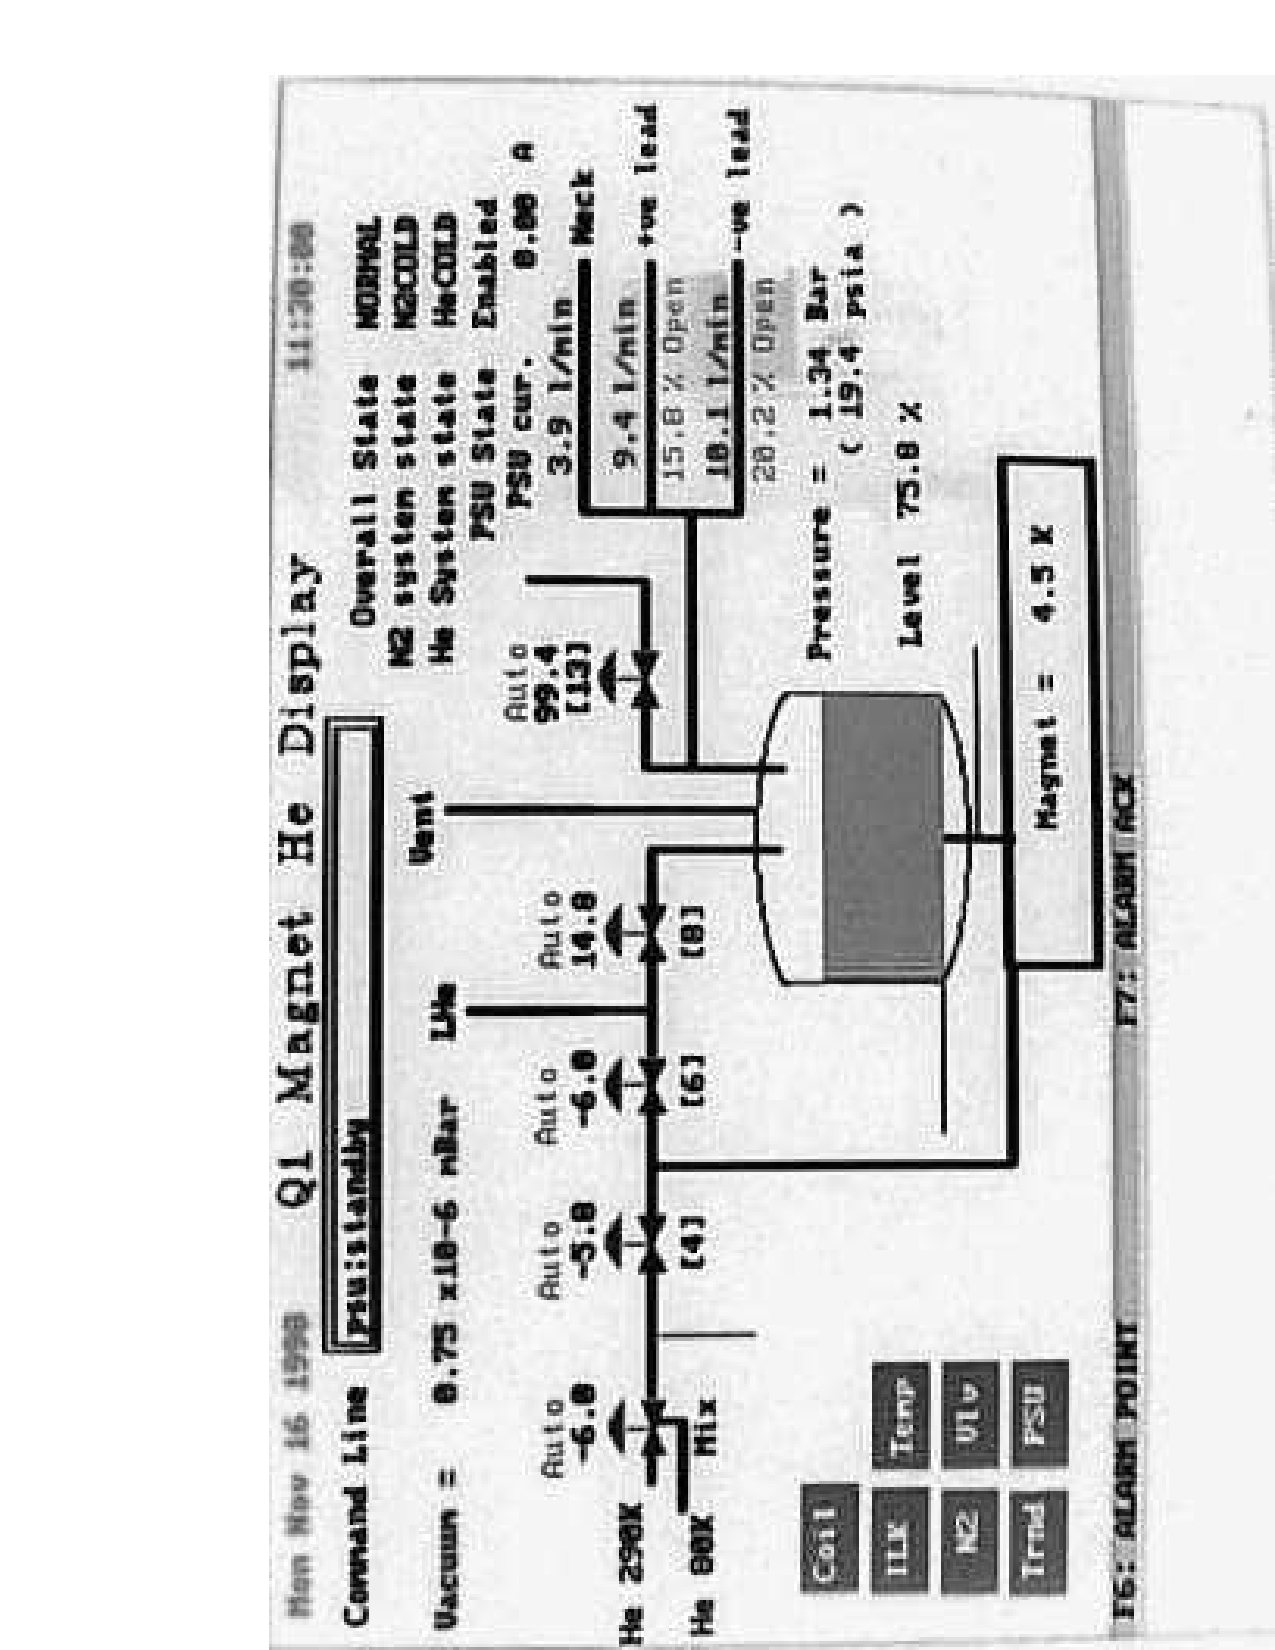
\includegraphics[angle=-90,width=4in]{Q1-helium}
\caption{Sample Helium Monitoring Page - Q1\label{fig:he_page}}
\end{figure}

\begin{figure}
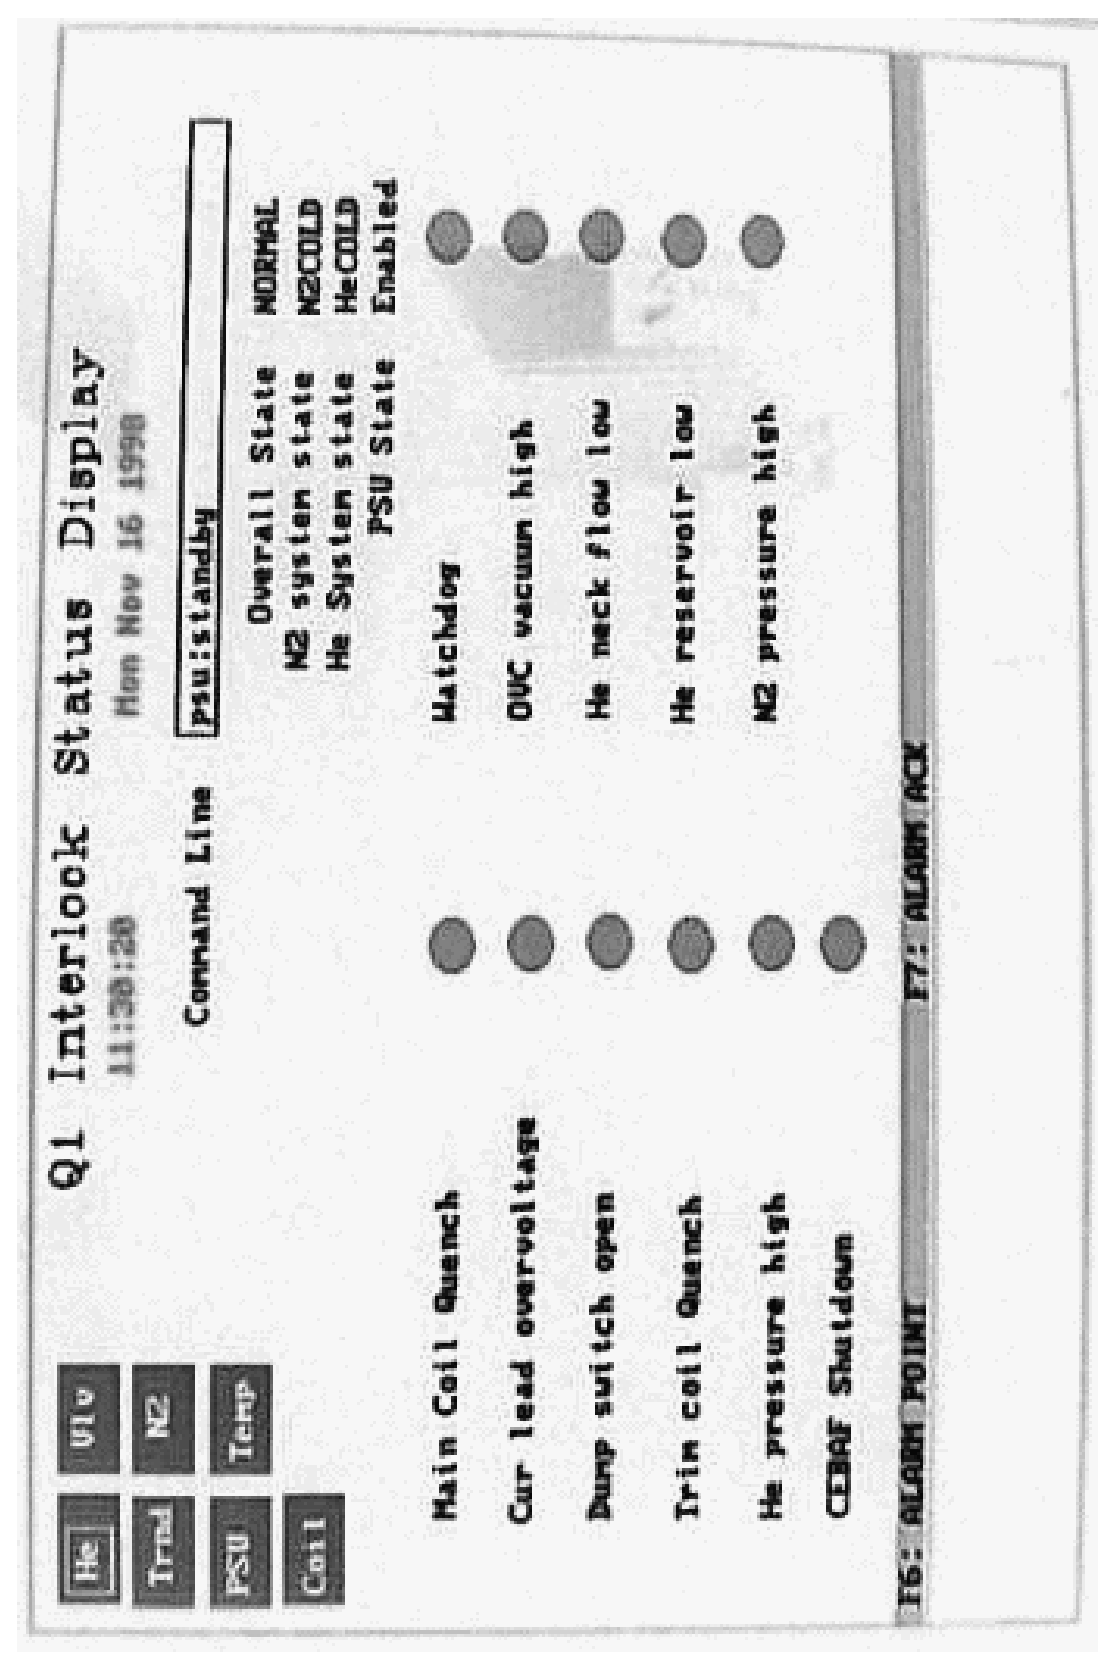
\includegraphics[angle=-90,width=4in]{Q1-interlock}
\caption{Sample Nitrogen Monitoring Page - Q1\label{fig:nit_page}}
\end{figure}

\begin{figure}
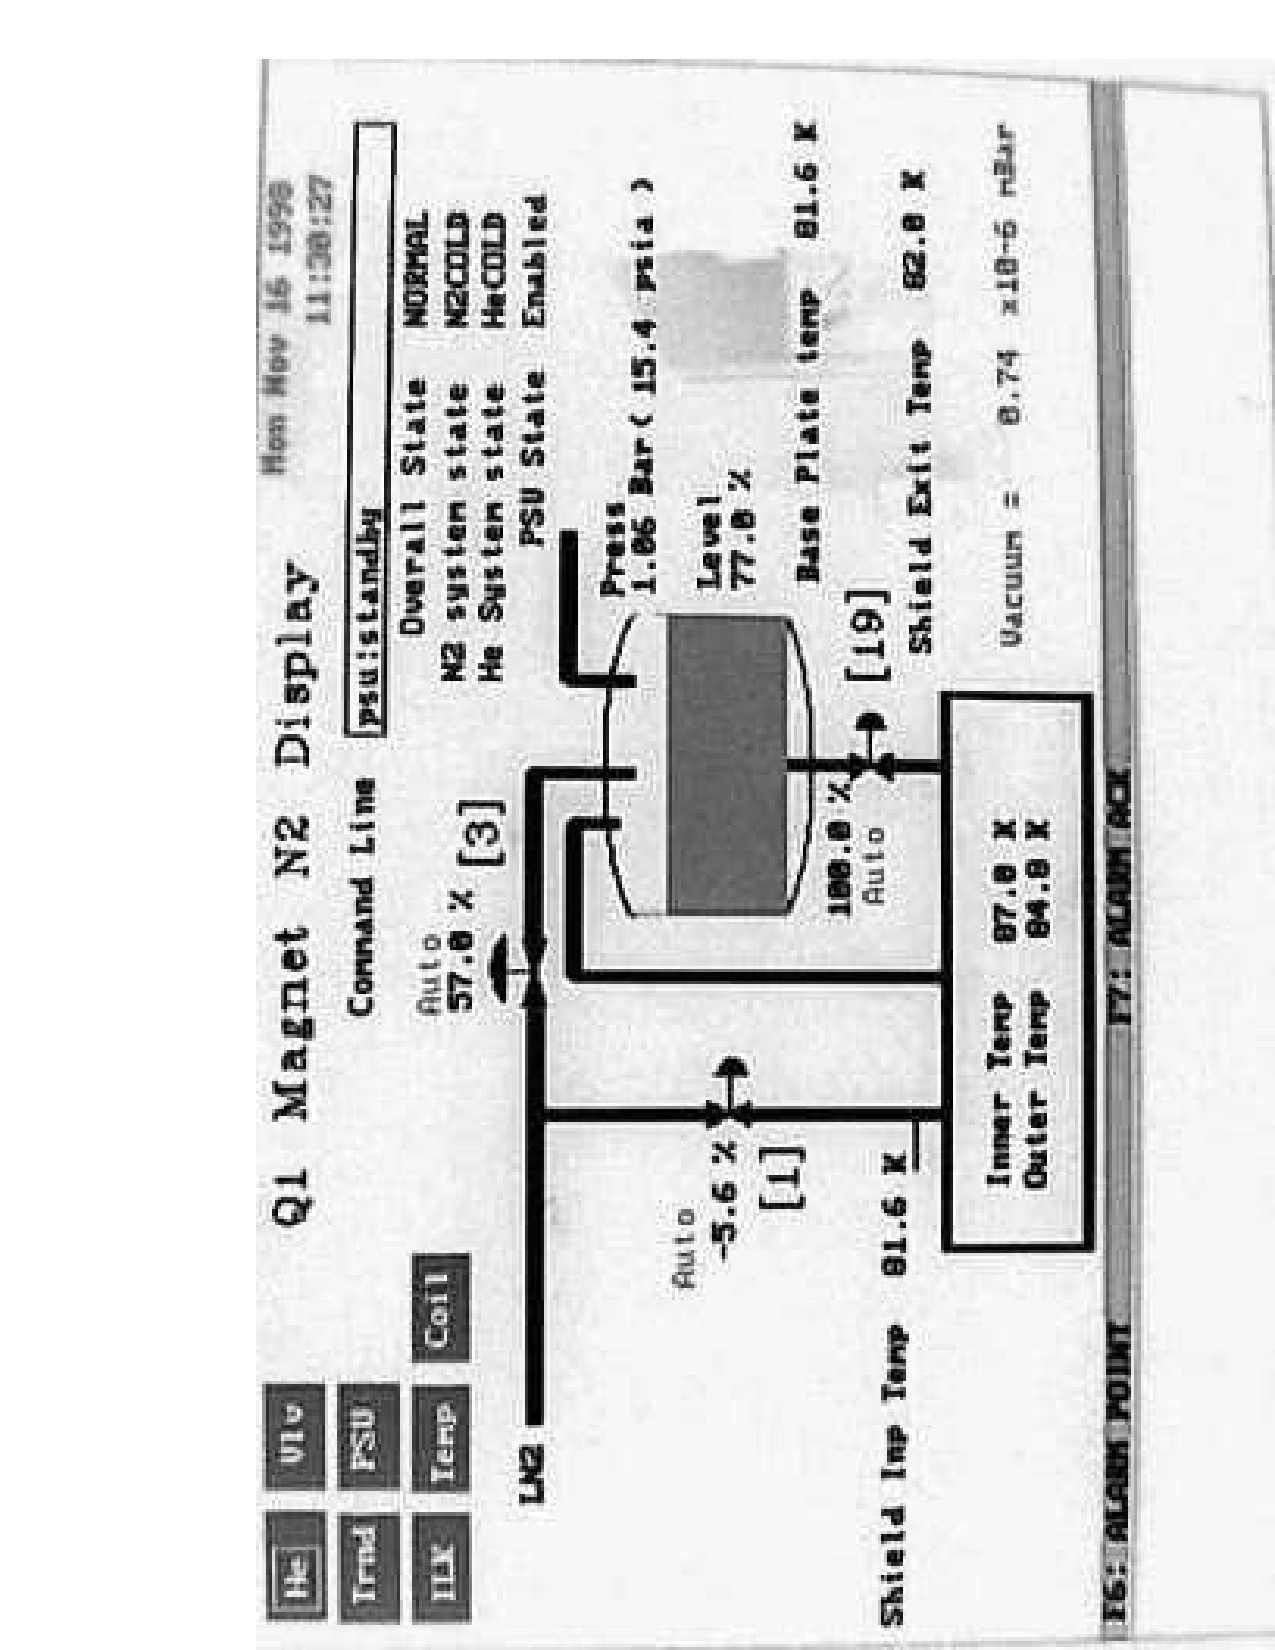
\includegraphics[angle=-90,width=4in]{Q1-n2}
\caption{Sample Power Supply Monitoring Page - Q1\label{fig:ps_page}}
\end{figure}

\begin{figure}
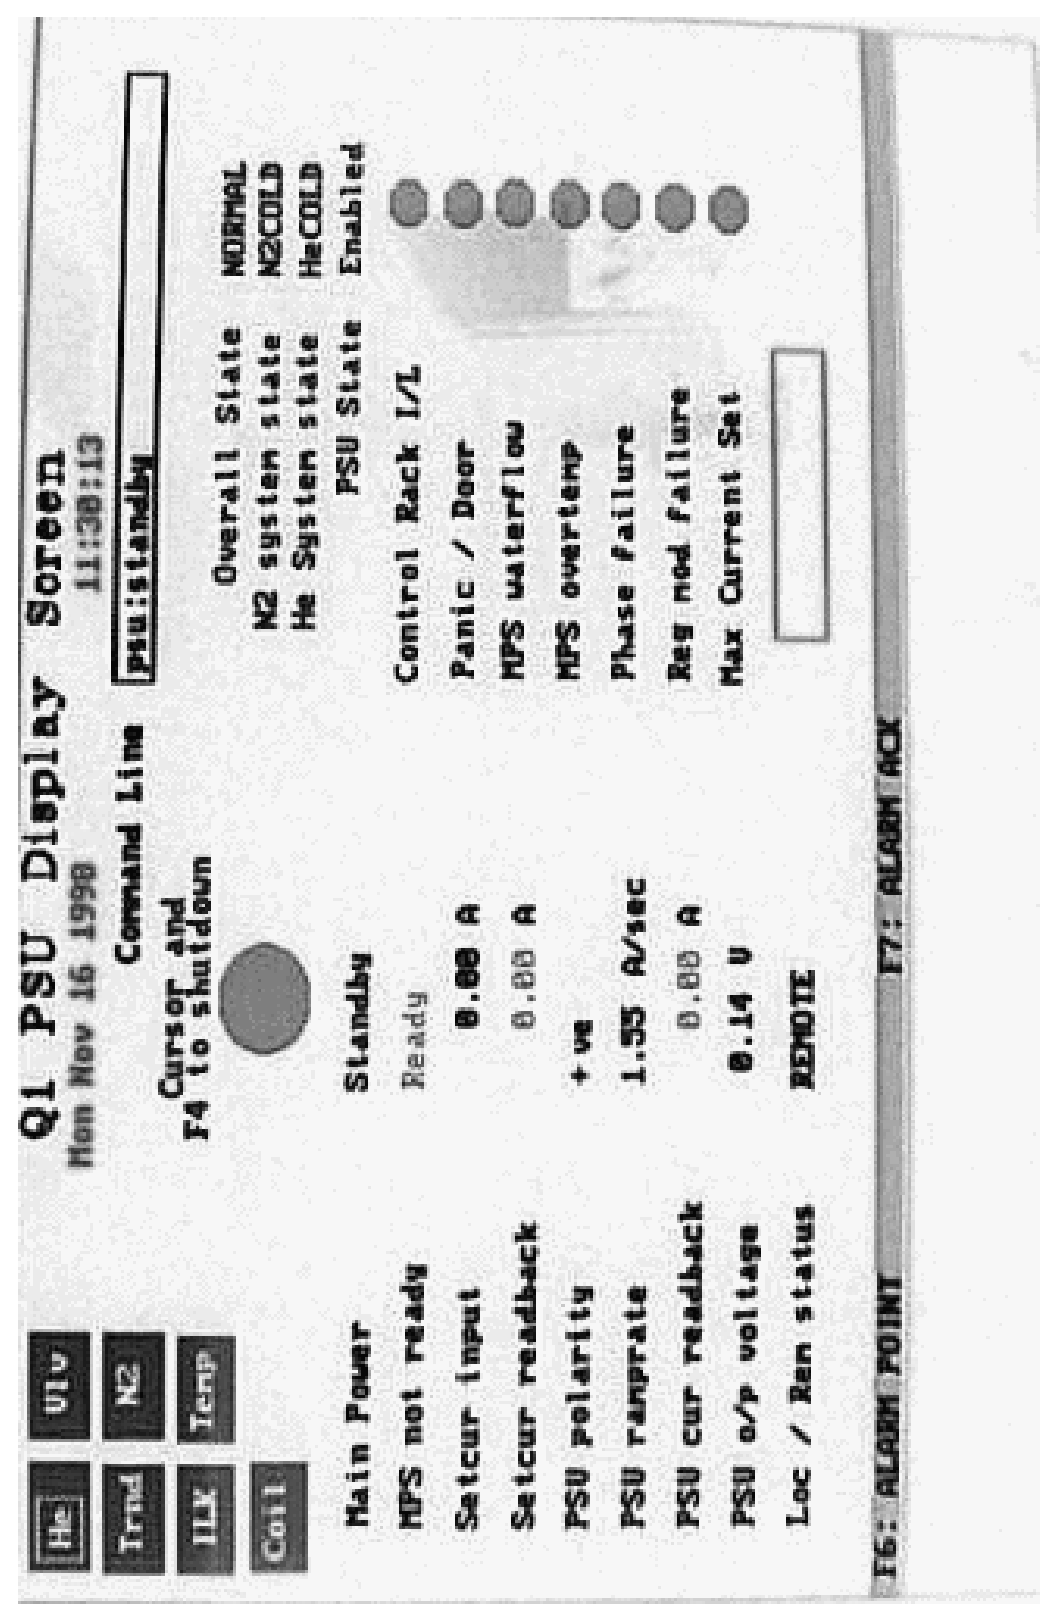
\includegraphics[angle=-90,width=4in]{Q1-psu}
\caption{Sample Interlock Monitoring Page - Q1\label{fig:is_page}}
\end{figure}

\begin{figure}
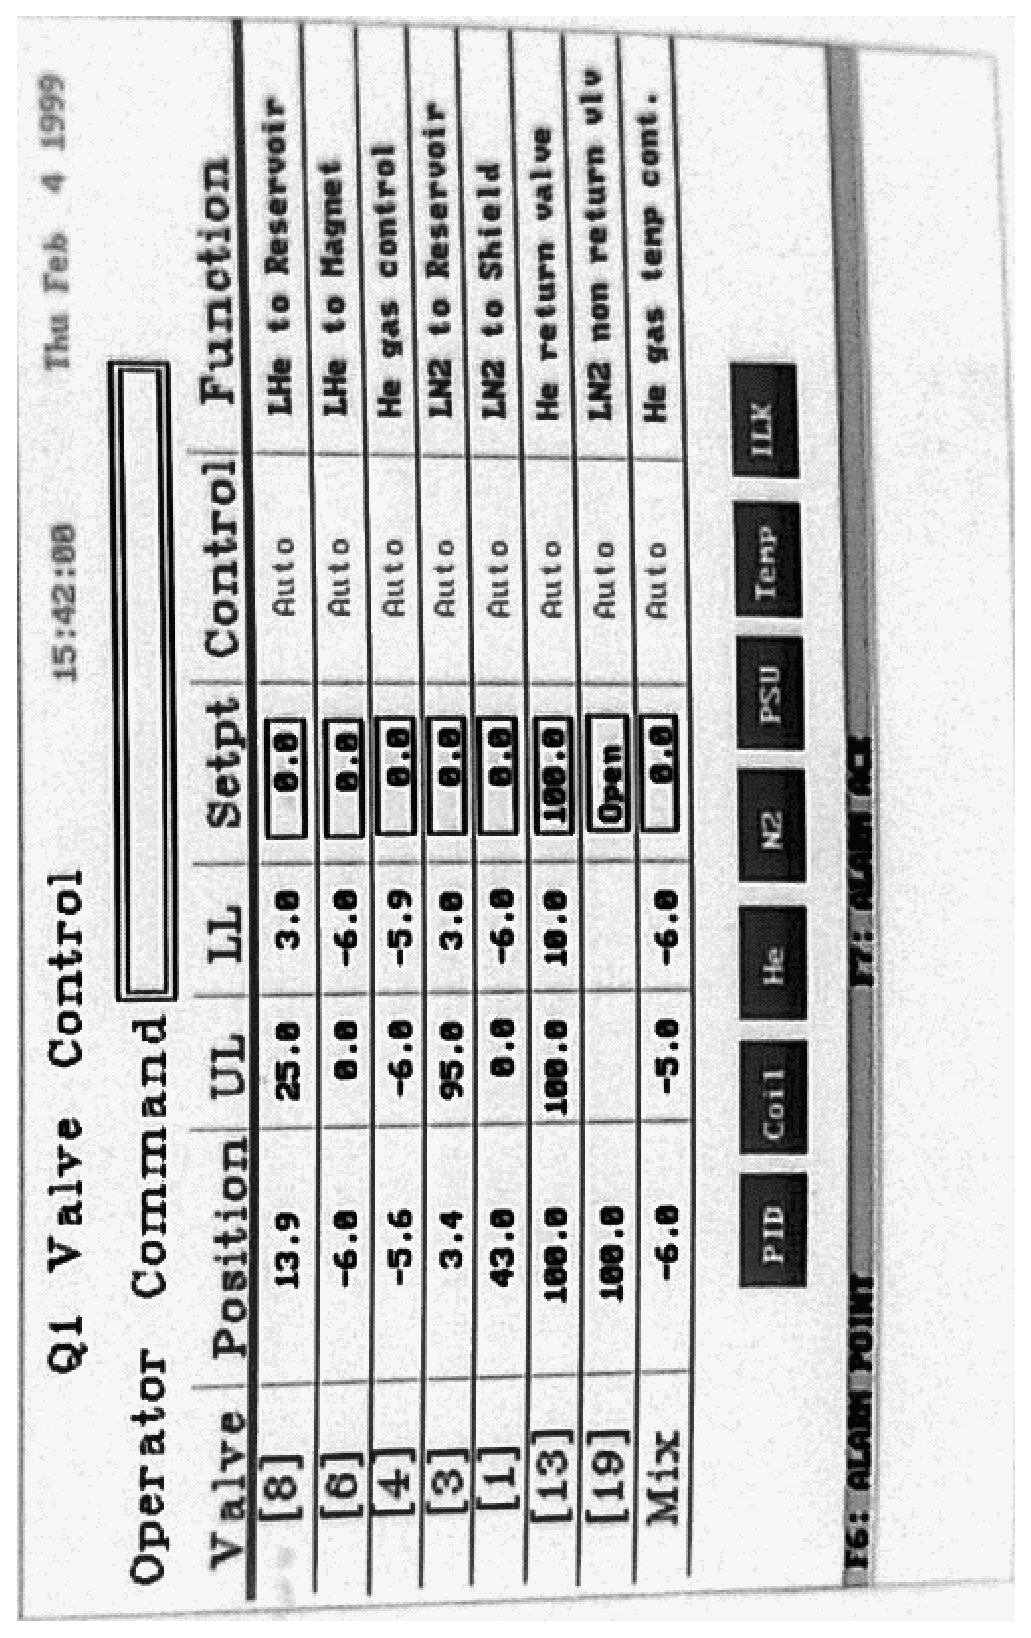
\includegraphics[angle=-90,width=4in]{Q1-valves}
\caption{Q1 Valve Control Page\label{fig:q1_valve_page}}
\end{figure}

%\begin{figure}
%\vspace{8.0in}
%\caption{Q1 Valve Control Page\label{fig:q2_valve_page}}
%\end{figure}

%\begin{figure}
%\vspace{8.0in}
%\caption{Q3 Valve Control Page\label{fig:q3_valve_page}}
%\end{figure}

\begin{figure}
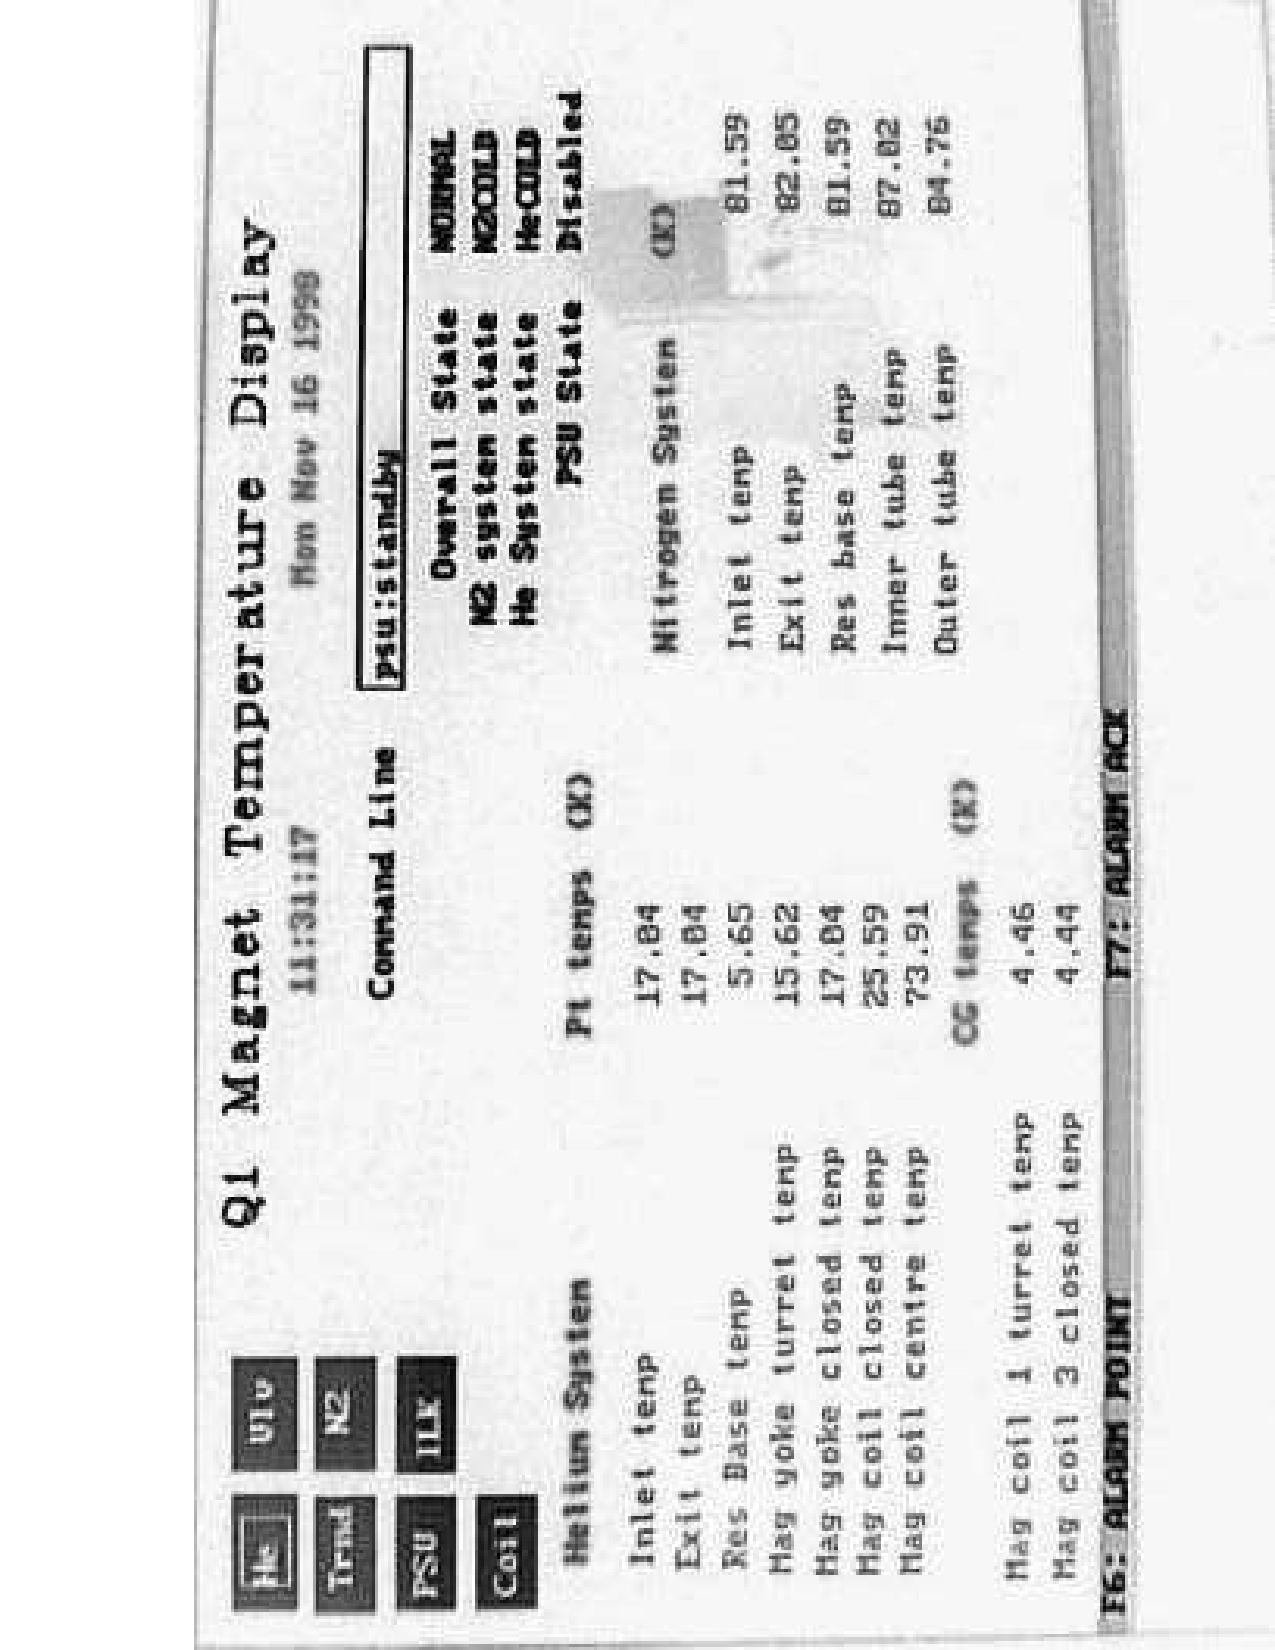
\includegraphics[angle=-90,width=4in]{Q1-temps}
\caption{Sample Magnet Temperature Display - Q1\label{fig:temp_page}}
\end{figure}

\begin{figure}
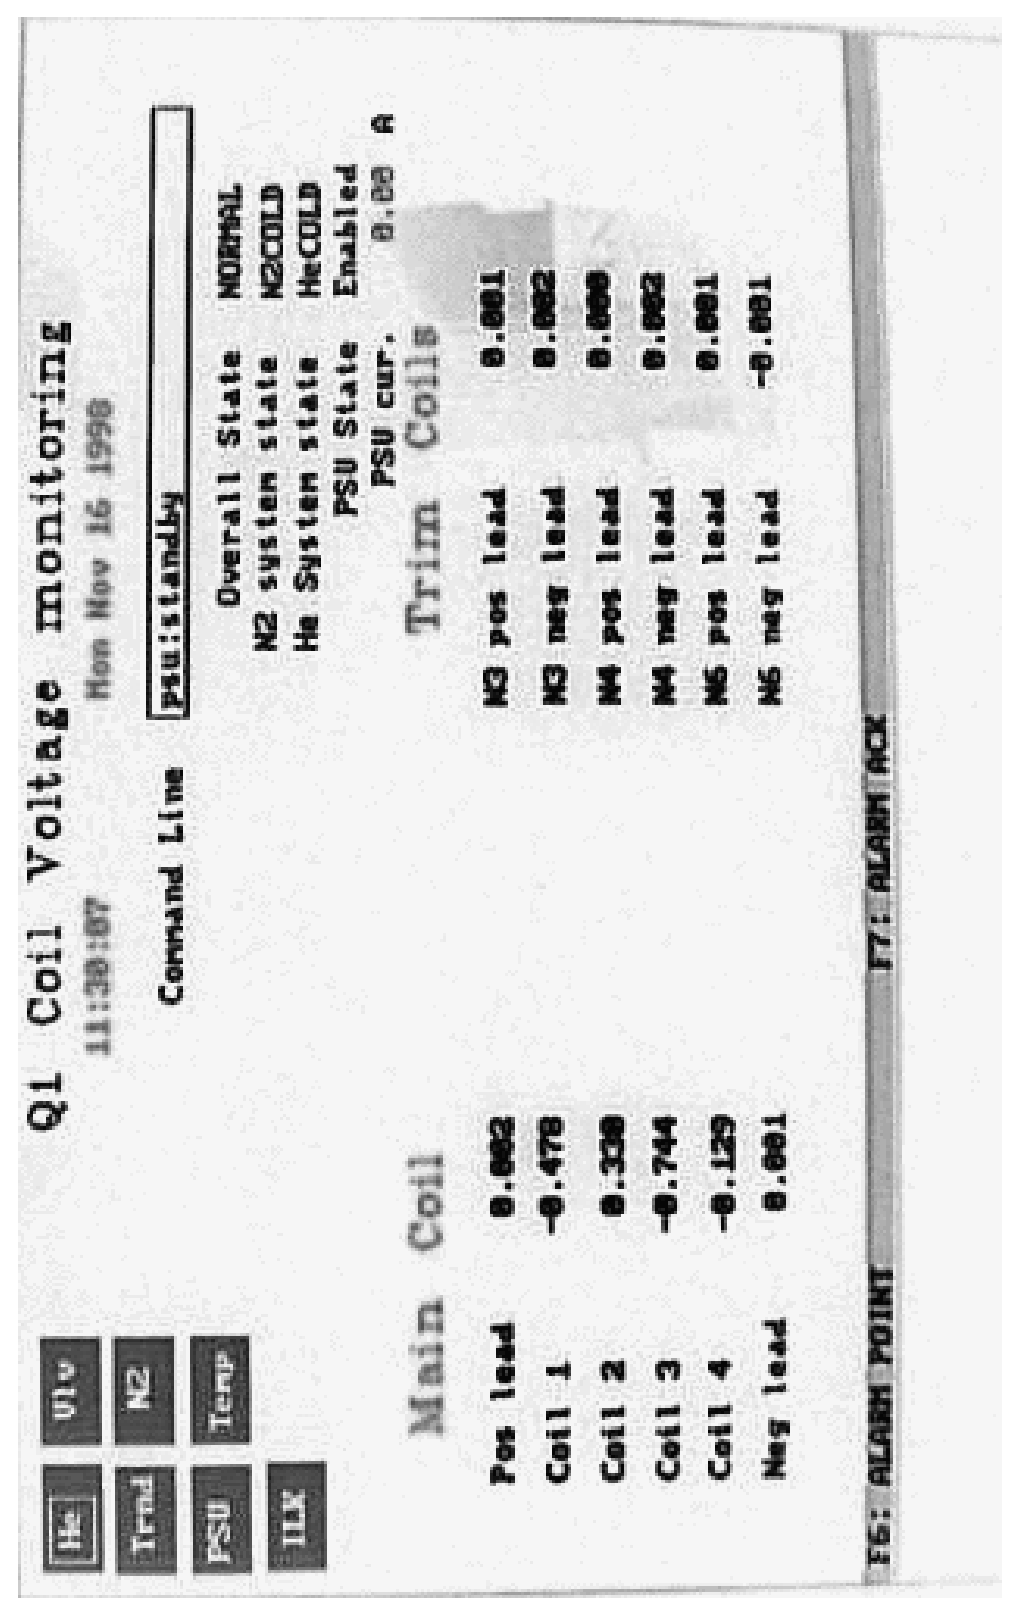
\includegraphics[angle=-90,width=4in]{Q1-voltage}
\caption{Sample Coil Voltage Monitoring Page - Q1\label{fig:coil_page}}
\end{figure}

\begin{figure}
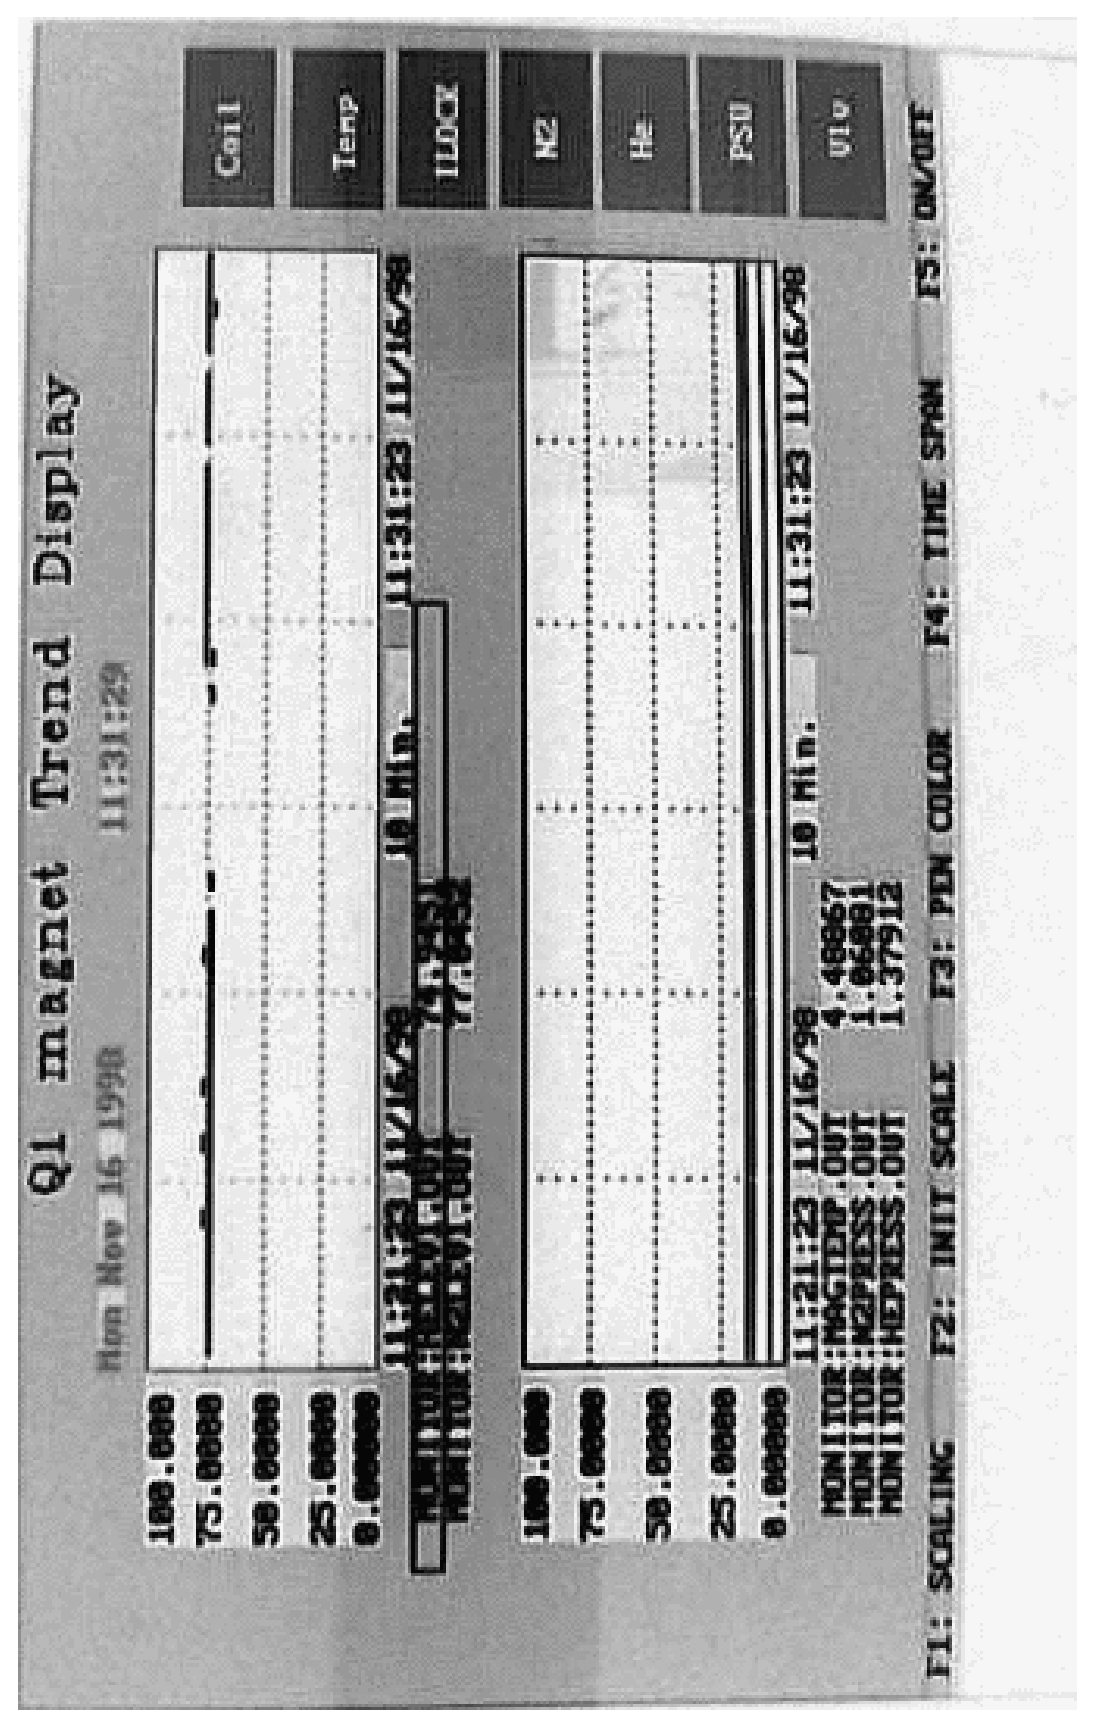
\includegraphics[angle=-90,width=4in]{Q1-trend}
\caption{Sample Trend Page\label{fig:trend_page}}
\end{figure}

\end{center}

\medskip

\begin{description}
\item[B.] {Dipole Pages}
\end{description}

\begin{description}
\item{}\hskip0.1in {[F1] Main Menu}
\item{}\hskip0.5in {Cooling (Cooldown Menu)}
\item{}\hskip0.5in {Field Regulation (NMR Controlled Programmed Ramp)}
\item{}\hskip0.5in {NMR Manual Operation (Field Control)}
\item{}\hskip0.5in {MPS Manual Operation (Current Control)}
\item{}\hskip0.1in {[F2] Coil Temperatures}
\item{}\hskip0.1in {[F3] Shield Temperatures}
\item{}\hskip0.1in {[F4] Cryogenic Page}
\item{}\hskip0.1in {[F5] Strain Gauge Page}
\item{}\hskip0.1in {[F6] Voltage Page}
\item{}\hskip0.1in {[F7] RS232 Status Page}
\end{description}

